\PassOptionsToPackage{full}{textcomp}
\documentclass[%
    a4paper, twoside, nobib%
]{tufte-book}
\hypersetup{colorlinks}

%%%%%%%%%%%%%%%%%%%%%%%%%%%%%%%%%%%%%%%%%%%%%%%%%%%%%%%%%%%%%%%%%%%%%%%%%%%%%%%
%% Metadata
\title{ML-based precision medicine in ischemic heart disease}
\author[Peter Christoffer Holm]{Peter Christoffer Holm}
\publisher{%
    Graduate School of Health and Medical Sciences
    University of Copenhagen%
}

%%%%%%%%%%%%%%%%%%%%%%%%%%%%%%%%%%%%%%%%%%%%%%%%%%%%%%%%%%%%%%%%%%%%%%%%%%%%%%%

\usepackage[%
    style=verbose-note,
    url=false,
    isbn=false,
    doi=false,
    eprint=false,
    date=year,
    maxcitenames=2,
    sorting=none,
    autocite=footnote,
]{biblatex}

\AtEveryCitekey{%
    \clearfield{pagetotal}%
    \clearfield{eprint}%
    \clearfield{pages}%
    \clearfield{series}%
    \clearlist{location}%
}
\addbibresource{assets/pch-thesis.bib}

%%%%%%%%%%%%%%%%%%%%%%%%%%%%%%%%%%%%%%%%%%%%%%%%%%%%%%%%%%%%%%%%%%%%%%%%%%%%%%%

\usepackage[p, osf]{ETbb} % osf in text, tabular lining figures in math
\usepackage[scaled=.95,type1]{cabin} % sans serif in style of Gill Sans

% \usepackage[varqu,varl]{zi4} % inconsolata typewriter

\usepackage{microtype}
\usepackage{booktabs}
\usepackage{lipsum}
\usepackage{pdfpages}
\usepackage{blindtext}
\usepackage{appendix}
\usepackage{amsmath}
\usepackage{amsfonts}
\usepackage{siunitx}
%\usepackage{cleveref}

\usepackage{todonotes}
\usepackage[inline]{enumitem}

\renewlist{enumerate*}{enumerate*}{1}
\setlist[enumerate*]{
    label=(\roman*), itemjoin={{; }}, itemjoin*={{; and }}
}

% quotation marks
\usepackage{csquotes}


% tikz %%%%%%%%%%%%%%%%%%%%%%%%%%%%%%%%%%%%%%%%%%%%%%%%%%%%%%%%%%%%%%%%%%%%%%%%
\usepackage{tikz}
\usetikzlibrary{positioning}
\usetikzlibrary{arrows,shapes}
\usetikzlibrary{quotes}
\usepackage{annotate-equations}


% For graphics / images
\usepackage{graphicx}
\setkeys{Gin}{width=\linewidth,totalheight=\textheight,keepaspectratio}
\graphicspath{{graphics/}}

% The fancyvrb package lets us customize the formatting of verbatim
% environments.  We use a slightly smaller font.
\usepackage{fancyvrb}
\fvset{fontsize=\normalsize}

% Hanging parentheses and asterisks
\newcommand{\hangp}[1]{\makebox[0pt][r]{(}#1\makebox[0pt][l]{)}}
\newcommand{\hangstar}{\makebox[0pt][l]{*}}

% Prints the month name (e.g., January) and the year (e.g., 2008)
\newcommand{\monthyear}{%
  \ifcase\month\or January\or February\or March\or April\or May\or June\or
  July\or August\or September\or October\or November\or
  December\fi\space\number\year
}

% Custom macros
\newcommand{\na}{\quad--}
\newcommand{\blankpage}{\newpage\hbox{}\thispagestyle{empty}\newpage}

%%%%%%%%%%%%%%%%%%%%%%%%%%%%%%%%%%%%%%%%%%%%%%%%%%%%%%%%%%%%%%%%%%%%%%%%%%%%%%%

\begin{document}
\frontmatter
\maketitle

\begin{@empty}
~\vfill
\thispagestyle{empty}
\setlength{\parindent}{0pt}
\setlength{\parskip}{\baselineskip}

\smallcaps{Candidate}

\textbf{Peter Christoffer Holm}, MSc

Novo Nordisk Foundation Center for Protein Research,
University of Copenhagen, Denmark

\smallcaps{Supervisors}

\textbf{Søren Brunak}, PhD, Professor 
(principal supervisor)

Novo Nordisk Foundation Center for Protein Research, 
University of Copenhagen, Denmark

\textbf{Henning Bundgaard}, PhD, Dr.Med, Professor 
(co-supervisor)

Department of Cardiology,
Copenhagen University Hospital, Denmark

\textbf{Karina Banasik}, PhD, Associate Professor 
(co-supervisor)

Novo Nordisk Foundation Center for Protein Research, 
University of Copenhagen, Denmark

\vspace{2em}

\par\smallcaps{Published by the \thanklesspublisher}

\vspace{5em}

\par This document was created using the \LaTeX{} typesetting software.
The layout is based on the \texttt{tufte-latex} document class,
and the main body of the text is set in \textsf{ETbb} and \textsf{Libertine}.
Unless otherwise indicated, all figures and graphics in the main text
are either the property of the author or are in the public domain.

%\par\textit{First printed, \monthyear}

Copyright \copyright\ \the\year\ \thanklessauthor
\end{@empty}

\begin{@empty}
\thispagestyle{empty}
\setlength{\parindent}{0pt}
\setlength{\parskip}{\baselineskip}

\chapter*{Preface}

This PhD thesis has been submitted
to the Graduate School of Health and Medical Sciences,
University of Copenhagen.

The work presented in this thesis was performed
at the Novo Nordisk Foundation Center for Protein Research (CPR),
University of Copenhagen, Denmark.

I declare no conflicts of interests.

\begin{flushright}
    Copenhagen, December 2023 \\
    Peter Christoffer Holm
\end{flushright}
\end{@empty}


\cleardoublepage

\setcounter{tocdepth}{1}
\listoftodos
\tableofcontents
\listoffigures
\listoftables
\cleardoublepage

%%%%%%%%%%%%%%%%%%%%%%%%%%%%%%%%%%%%%%%%%%%%%%%%%%%%%%%%%%%%%%%%%%%%%%%%%%%%%%%

\mainmatter

\chapter{Summary}

\chapter{List of Manuscripts}
\section{Manuscripts included in this thesis}
\subsection{Paper 1}

Amalie D. Haue*, 
\underline{Peter C. Holm}*, 
\marginnote{%
  An asterisk (*) denotes equal contribution.

  \noindent
  This manuscript was also included in the thesis of Amalie D. Haue.
}
Karina Banasik, Agnete T. Lundgaard, Victorine P. Muse, Timo Röder, 
David Westergaard, Piotr J. Chmura, Alex H. Christensen, Peter E. Weeke, 
Erik Sørensen, Ole B. V. Pedersen, Sisse R. Ostrowski, Kasper K. Iversen, 
Lars V.  Køber, Henrik Ullum, Henning Bundgaard, 
and Søren Brunak:
\textbf{\enquote{%
    Subgrouping multimorbid patients with ischemic heart disease 
    by means of unsupervised clustering: 
    A cohort study of 72,249 patients 
    defined comprehensively by diagnoses prior to presentation
}}.
\textit{%
    Submitted for publication (under review).
    Preprint posted on medRxiv (2023): 2023-03.
}

\subsection{Paper 2}
\underline{Peter C. Holm},
\marginnote{%
  An ealier version of this  manuscript was included in the thesis of 
  Amalie D. Haue.%
}
Amalie D. Haue,  
David Westergaard, Timo Röder, Karina Banasik, Vinicius Tragante, 
Alex H. Christensen,  Laurent Thomas,  Therese H. Nøst, Anne-Heidi Skogholt, 
Kasper K. Iversen, Frants Pedersen, Dan E. Høfsten, Ole B. Pedersen,  
Sisse Rye Ostrowski, Henrik Ullum, Mette N. Svendsen, Iben M. Gjødsbøl, 
Thorarinn Gudnason, Daníel F. Guðbjartsson,  Anna Helgadottir, Kristian Hveem,  
Lars V. Køber,  Hilma Holm, Kari Stefansson,  Søren Brunak,  
and Henning Bundgaard:
\textbf{\enquote{%
    Development and validation of a neural network-based survival model 
    for mortality in ischemic heart disease%
}}.
\textit{%
    Submitted for publication (under review).
    Preprint posted on medRxiv (2023): 2023-06.
}

\subsection{Paper 3}
\underline{Peter C. Holm},
\todo{add more authors once manuscript is ready}
\ldots, Henning Bundgaard, and Søren Brunak
\enquote{%
    Development of a neural network-based competing risk model 
    for individualized prognostication in ischemic heart disease 
    using a large database of electronic health records 
    and clinical registries}
preprint: \textit{medRxiv (2023): 2023-12.}

\clearpage
\section{Manuscripts not included in this thesis}

\subsection{Paper 4}
Isa K. Kirk, \ldots, 
\underline{Peter C. Holm},
\ldots, Søren Brunak
\textbf{\enquote{%
    Linking glycemic dysregulation in diabetes to symptoms, 
    comorbidities, and genetics through EHR data mining
}}
in \textit{eLife} (2019)

\subsection{Paper 5}
Ina H. Laursen, \ldots, 
\underline{Peter C. Holm},
\ldots, Henrik Ullum
\textbf{\enquote{%
    Cohort profile: Copenhagen Hospital Biobank - Cardiovascular Disease Cohort
    (CHB-CVDC): Construction of a large-scale genetic cohort to facilitate a
    better understanding of heart diseases
}}
in \textit{BMJ Open} (2021)

\subsection{Paper 6}
Amalie D. Haue, \ldots, 
\underline{Peter C. Holm},
\ldots, Henning Bundgaard, and Søren Brunak
\textbf{\enquote{%
    Temporal patterns of multi-morbidity in 
    570157 ischemic heart disease patients: 
    a nationwide cohort study
}}
in \textit{Cardiovascular Diabetology} (2022)

\subsection{Paper 7}
Alex W. Jung, 
\underline{Peter C. Holm}, \ldots, 
Søren Brunak, and 
Moritz Gerstung
\textbf{\enquote{%
    Multi-cancer risk stratification based on national health data: a
    retrospective modelling and validation study
}}
preprint in \textit{medRxiv} (2022)

\subsection{Paper 8}
Karina Banasik, \ldots, 
\underline{Peter C. Holm}, \ldots, 
Thomas F. Hansen
\textbf{\enquote{%
    DanMAC5: a browser of aggregated sequence variants from 8,671 whole genome
    sequenced Danish individuals
}}
in \textit{BMC Genomic Data} (2023)

\subsection{Paper 9}
David Westergaard, \ldots, 
\underline{Peter C. Holm}, \ldots, 
Søren Brunak, and 
Henriette S. Nielsen
\textbf{\enquote{%
    Immune Changes in Pregnancy: Associations with Pre-existing Conditions and
    Obstetrical Complications at the 20th Gestational Week-A Prospective Cohort
    Study
}}
preprint in \textit{medRxiv} (2023)



%%%%%%%%%%%%%%%%%%%%%%%%%%%%%%%%%%%%%%%%%%%%%%%%%%%%%%%%%%%%%%%%%%%%%%%%%%%%%%%

\chapter{Thesis Objectives and Overview} \label{intro}

The overall aim of this thesis is ...


\vskip 10em

With the advent of large language models (LLMs) like ChatGPT
%------------------------------------------------------------------------------
\marginnote{%
    \textsf{hype}, (noun). [clipping of hyperbole].

    (marketing) promotion or propaganda; especially exaggerated claims. 
    \rightline{\textit{wiktionary.org}}%
}
%------------------------------------------------------------------------------
and text-to-image models such as DALL-E and Midjourney,
there has been a surge of interest in the broader domains of
artificial intelligence and machine-learning.
%
ChatGPT, in particular, stands out as prominent example---%
an LLM-based chatbot developed by OpenAI, 
have managed to impress both the general public aswell 
as researchers across various disciplines.
It has been shown that ChatGPT can pass exams
such as USMLE\footnotemark
~\autocite{openaiGPT42023}

%------------------------------------------------------------------------------
\footnote{%
The United States Medical Licensing Examination (USMLE) 
is a three-step examination program for obtaining a medical license
in the United States of America.
}
%------------------------------------------------------------------------------






It has been claimed that 




However, 




The convergence of precision medicine and artificial intelligence 
stands as a monumental paradigm shift, promising to redefine
the way we diagnose, treat, and manage disease.



It is this author's opinion, 
that the main cause of \enquote{success} of the abovementioned
AI-applications is the combined value of 
absolutelive massive datasets and massive computing power.

This thesis has little to do with the likes of ChatGPT, 
but 

In this thesis, I explore how data-drive approaches
can further the development of precision medicine in ischemic heart disease.

The thesis is structured as follows:
in the chapter \nameref{precision-medicine} I will be introducing the 
concept of precision medicine framed in the context of \enquote{big data}
and \enquote{machine learning}.

In \nameref{ml-fundamentals}

In \nameref{survival-analysis}

In \nameref{results}

In \nameref{conclusions}




Although we in the three manuscripts that forms this thesis 
primarily place a focus on cardiology,
and specifically ischemic heart disease,
the presented methods can be used across many fields of medicine.




\chapter{Ischemic Heart Disease}
\label{ihd-background}

Ischemic heart disease is a term covering a variety of conditions, 
all caused by myocardial ischemia---%
an imbalance between the coronary blood supply and the 
oxygen requirements of the myocardium.
In the overwhelming majority of cases, 
this imbalance can be attributed to obstructive atherosclerotic disease 
that limits coronary blood flow
~\autocite{kumarRobbins2017}.
In these cases, ischemic heart disease is therefore synonymous 
with coronary artery disease.

The central etiological entity in ischemic heart disease
is therefore the atherosclerotic plaque, 
which is part of the process known as atherosclerosis. 
An atherosclerotic plaque consists of blood cells, lipids, calcium 
and connective tissue that are gradually deposited in the arterial wall 
over a number of years.
~\autocite{kumarRobbins2017}
The plaque can grow large enough to severely narrow the arterial lumen,
or it can become unstable and as a consequence rupture or erode,
leading to thrombosis.
Both of these scenarios can severely affect 
the perfusion of tissues and organs, 
and when coronary arteries are affected,
it can lead to ischemic heart disease.

\begin{figurefw}
    \centering
    \vspace{-5em}
	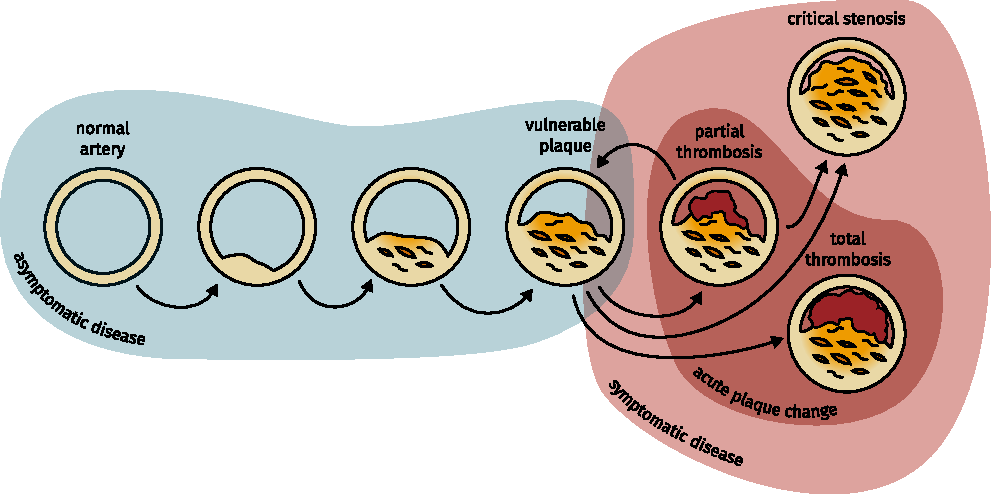
\includegraphics[width=\linewidth]{graphics/atherosclerosis}
    \caption[The process of atherosclerosis]{%
        \textit{Critical stenosis} represents the tipping point at which
        the gradual occlusion of the arteries leads to onset of symptoms.
        While the patient may be asymptomatic at rest, 
        increased physical activity results in cardiac ischemia and  
        intense chest pain.
        \textit{Acute plaque change} is the sudden rupture or erosion of 
        the atherosclerotic plaque which triggers thrombosis.
        The resulting thrombus can partially or completely fill the vascular
        lumen.
        Disruption of endothelial integrity.
    }
    \label{OneOfMyMissingFigures}
\end{figurefw}

\vskip 10em
%------------------------------------------------------------------------------

\section{Manifestation}

The underlying pathological process is inherently chronic,
but ischemic heart disease can abruptly transition to an acute condition.
Often, the disease is initially identified when this acute transition 
has already happened.




The clinical presentation of ischemic heart disease include
both chronic and acute manifestations of myocardial ischemia. 

\begin{table}
    \begin{tabular}{ll}\toprule
        Syndrome              & Manifestation \\\midrule
        Angina Pectoris       & Description \\
        Myocardial Infarction & Description \\\bottomrule
    \end{tabular}
\end{table}




\section{Prevalence}

\todo[inline]{Danish statistics on IHD incidence and prevalence.}



Angina pectoris, myocardial infarction, chronic IHD, and sudden cardiac death.

Chronic ischemic heart disease is a syndrome characterised by
gradual heart failure following ischemic myocardial injury.

Inflammation.
Endothelial cells and circulating leukocytes.
T-cell and macrophage recruitment and activation.
Smooth muscle cell accumulation. 



Typical or stable angina is episodic but consistent chest pains
linked to physical activity.
Unstable angina, is as its name indicate more variable, and 
is usually characterized by an increase in frequency and intensity
of chest pain.

Myocardial infarction is caused by acute thrombosis following 
sudden ruption or erosion of an atherosclerotic plaque.



The central entity in the etiology of ichemic heart disease 
is the atherosclerotic plaque. 

Fate of the atherosclerotic plaque



Atherosclerotic plaques can, 
as they increase in size, occlude the vascular lumen 
and mechanically affect the circulation.


In coronary atherosclerosis, 
The abnormal, often turbulent, blood flow in the vicinity of atherosclerotic
plaques can, in combination with the loss of endothelial integrity, lead to
formation of arterial thromboses.
~\autocite{kumarRobbins2017}

Such thromboses can embolise, but may also increase in size and gradually 
occlude the vascular supply of the heart.
The consequences of the occlusion can,
depending on the local vascular anatomy and extent of the occlusion,
range from relatively benign to extensive tissue necrosis
and even death~\autocite{kumarRobbins2017}.

\section{Consequences and Complications}
\section{Co-morbidity}
\section{Diagnosis}
\section{Complications}
\section{Treatment}

If the occlusion of one coronary artery happens slowly, 
it can allow time for the development of collateral blood supplies,
which might prevent myocardial infarction
~\autocite{kumarRobbins2017}.


\chapter{Data-driven Precision Medicine} \label{precision-medicine}

A 2013 Cochrane review on \citetitle{taylorStatins2013} concluded 
that statins effectively lower all-cause mortality and reduce the incidence
of both fatal and non-fatal cardiovascular events all without any serious
adverse effects~\autocite{taylorStatins2013}.
For instance, the relative risk of fatal cardiovascular events 
when using statins as opposed to placebo
was estimated to \num{0.82} with a 
\si{95}{\%} \ac{CI} of \num{0.70} to \num{0.96}.
~\autocite{taylorStatins2013}
This means that those treated with statins, on average,
are \si{18}{\%} less likely to die from cardiovascular causes. 
However, it is important to emphasize that this \si{18}{\%} 
reduction is an average effect.
There might be groups of people for whom the reduction could be 
even higher, while others may see little to no benefit. 
Understanding and making use of such individual variability 
is the central objective of precision medicine.

As a concept, precision medicine is not a new idea;
tissue- and blood typing, for instance,  
has been used to guide treatment for many decades.
However, the prospective of leveraging large clinical databases
and broad array of phenotypic information 
to deliver precision medicine across
a wide spectrum of disease states
is adding renewed interest in the concept.






Use data to improve decision making


Subgroup identification seeks to identify groups of individuals with an
increased treatment response, which
\citeauthor{kosorokPrecision2019} refers to as 
\textquote[kosorokPrecision2019]{%
    finding the right patient for the right treatment%
}.


\begin{table*}[h]
    \footnotesize
    \centering
    \begin{tabularx}{0.9\textwidth}{XlX} \toprule
    Condition & Gene & Action \\
    \midrule
    Familial hypercholesterolaemia & \textit{PCSK9}, \textit{APOB}, and \textit{LDLR} & Indication for PCSK9 inhibitor drugs \\
    Familial hypercholesterolaemia & \textit{PCSK9}, \textit{APOB}, and \textit{LDLR} & Indication for PCSK9 inhibitor drugs \\
    Familial hypercholesterolaemia & \textit{PCSK9}, \textit{APOB}, and \textit{LDLR} & Indication for PCSK9 inhibitor drugs \\
    Familial hypercholesterolaemia & \textit{PCSK9}, \textit{APOB}, and \textit{LDLR} & Indication for PCSK9 inhibitor drugs \\
    Chronic myeloid leukemia       & BCR/ABL & Imatinib \\
    Chronic myeloid leukemia       & BCR/ABL & Imatinib \\
    Chronic myeloid leukemia       & BCR/ABL & Imatinib \\
    Chronic myeloid leukemia       & BCR/ABL & Imatinib \\
    Chronic myeloid leukemia       & BCR/ABL & Imatinib \\
    \bottomrule
    \end{tabularx}
    \caption[Precision drugs]{
        Examples of precision pharmacotherapy informed by genetics 
        and more more more more
    }
\end{table*}



Electronical health records are a rich source of health data,
and can be used to find connections between risk factors and diseases.

Precision medicine is prevention and treatment approaches
that takes individual variation into account.


The terms
\enquote{precision},
\enquote{personalized},
and \enquote{individualized medicine}
are often used interchangeably.






\section{Deep phenotyping} \label{deep-pheno}

In their review 
\citetitle{konigWhat2017}, 
\citeauthor{konigWhat2017} presents data-driven precision medicine
as a framework with three main \enquote{tracks} or \enquote{processes}
that serves as an useful abstraction for understanding
the process of moving from big data
to clinically actionable insights~%
\autocite{konigWhat2017}. 
At the center of the framwork resides the data,
which are both plentiful and representative of the population of interest.
Now, the three tracks are
1) preprocessing and data-mining
2) diagnostic and prognostic models
and 3) prediction of treatment response.

\subsection{Track 1: preprocessing and data mining}

Quality control, preprocessing, and extraction of information.
The concrete steps and methods utilized as part of this track
is highly context-dependent, 
and is therefore difficult to describe on a general level. 

Feature-engineering.

Extracting structured information from unstructured information.

Clustering.

\subsection{Track 2: diagnostic and prognostic models}

Relying in part on processed data from track 1
as well as any insights gained from data-mining,
track 2 is concerned with the development
of models that can characterise current (diagnostic models)
or future (prognostic models) states of health and disease~%
\autocite{konigWhat2017}. 

\subsection{Track 3: predicting treatment response}

\todo[inline, caption={Some text}]{
\begin{minipage}{\linewidth}
    \emph{Notes:}

    Causality.
    Different strategies exists for guiding the development of 
    predicting therapy response.
    We might be able to use prognostic and diagnostic factors
    discovered in the previous track to predict treatment response.
    Example: HER is prognostic for survival in breast cancer,
        but is also predictive of treatment response against X.


\end{minipage}
}

As with the other tracks, track 3 gan generate further knowledge 
that in turn can feed back to the more general phenotyping of patients
\autocite{konigWhat2017}. 


\section{Health Informatics}

Health informatics is a cross-disciplinary field
that aims at developing methods and techniques
for the collection, study, and analysis of healthcare data.
It operates in the intersection between medicine and computer science,
and involves disciplines such as
bioinformatics, software engineering, statistics, information systems,
data science, and artificial intelligence.
The overall goal of health informatics is the data-driven improvement
of delivery and accuracy of health and healthcare for the individual patient.

In modern medicine, 
ever increasing amounts of data 
is continuously being generated and collected.
Ranging from structured administrative data 
used primarily for billing purposes
to advanced imaging and high-througput \enquote{omics} analyses,
the array of available data is as diverse as it is plentiful.

The volume and range of information collected
at just a single visit for a single patient
can be large.


There is increasing evidence that informatics improves
health care, public health, and biomedical research.

    
An electronic health record
is a systematized collection of health data 
stored in a digital format.
Electronic health records may include data such as
medical history, drug prescriptions, laboratory test results,
radiology images, body measurements, and billing information.
EHRs enable following patients in both time and space;
not only in the physical space that is the cardiology department
and the intensive care unit, but also in the health-and-disease space.

\begin{itemize}
    \item \textbf{Decision support systems}
    \item \textbf{Personalized medicine}
    \item \textbf{Mobile health applications} (aka. \textit{mHealth})
    \item \textbf{Screening}
    \item \textbf{Surveillance}
    \item \textbf{Medical outcomes}
\end{itemize}

\marginnote{
    The five Vs of big data:
    \begin{itemize}
        \item Volume
        \item Velocity
        \item Variety
        \item Value
        \item Veracity
    \end{itemize}
}

\section{Clinical decision support systems}

Deep learning can identify patterns in sparse, noisy,
and very heterogenous data without the need for expert feature engineering
\cite{norgeotCall2019}.

Challenges in developing machine learning models from electronic health records
includes syntactic interoperability, 
which specifies the format and structure of the data.
Many different interopability formats exists, 
but their adoption varies considerably.

Benefits of interopable digital health data
~\autocite{lehneWhy2019}.
Test~\cite{lehneWhy2019}.

\begin{itemize}
    \item Large-scale observational studies.
    \item Less time spend on data cleaning and pre-processing.
    \item Interoperable exchange format could further cross-institutional
    and international collaboration, which would make it easier 
    to reproduce and externally validate e.g. prognostic applications.
    In the case of rare diseases with very limited number of patients, 
    international pooling of data could enable analysis
    that otherwise would not be possible.
    \item Faster research and development process.
    \item If data is known to conform to a well-defined format,
    computer software can be written without explicit access to the data.
    This solve many issues related to sensitive data or
    data that are otherwise subject to strict data protection regulations.
\end{itemize}


Healthcare data are usually private and scattered across various applications,
which makes it difficult to share data and generate robust results 
that translate to different and diverse populations.


Succesful implementation of data-driven applications
require large and diverse data sets.

AI approaches rely on data that accurately represent
the real-life distribution of the underlying problem.
We can not exclusively rely on data that have been carefully curated 
from few and often very similar sources. 
In order to capture subtle relationships 
between health and disease patterns,
we need to include many and diverse cases~%
\autocite{riekeFuture2020}.

Federated learning could solve some of these issues\autocite{riekeFuture2020}.





\chapter{Machine Learning}

The promise of AI lies in the ability 
to integrate large amounts of data from huge data sets
and almost instantaneously register patterns
with clinical importance.

Machine Learning seeks to let computers learn from data
without them being explicitly programmed.


The Turing test, proposed by Alan Turing in 1950,
tries to answer the question \enquote{can a machine think?}.
A computer passes the test if a human interogator,
after posing a series of written questions,
cannot determine if the responses come from a human or a computer.


\textquote[\autocite{russellArtificial2009}]{%
The quest for \enquote{artificial flight} succeeded 
when engineers and inventors stopped imitating birds 
and started using wind tunnels and learning about aerodynamics.
Aeronautical engineering texts 
do not define the goal of their field as making 
\enquote{machines that fly so exactly like pigeons 
that they can fool other pigeons.}\,}

If the output is a finite set of values
the learning problem is called \textbf{classification},
and if it is a number, then it is called \textbf{regresion}.

In supervised learning, the model observes input-output pairs
and tries to learn a function that maps inputs to outputs.

In unsupervised learning, the model learns patterns in unlabeled input data.

With many machine-learning models, there is a bias--variance tradeoff:
on one end of the spectrum we have simple low-variance models 
such as linear or logistic regression
and on the other end, we have high-variance models
such as neural networks or random forests.

We can estimate the error rate of model
by evaluating it on a test set.
If we are only creating a single model,
then this approach suffices. 
However, we might want to compare many different models,
or slightly tweak an already existing model,
such that we can select the performing version.
If we select the final model based on the test set,
we might inadvertently have biased the process,
and could, in a sense, have overfitted to the test data.
To avoid this, we need to completely hide away the test data
until we are done with training, experimenting, 
and hyperparameter optimization.
To allow this, we instead need three sets of data:

\begin{itemize}
    \item a training set to train or develop candidate models
    \item a validation set to evaluate the candidate models
        and select the best one
    \item a test set do the final unbiased evaluation of model performance
\end{itemize}

Another alternative is using the technique \textit{k}-fold cross-validation.

A model is interpretable if we can inspect the model
and understand why it gave a certain output for a particular input.
An explainable model is one that can help us understand 
why a certain output was produced for a specific input.
Interpretability comes from inspecting the actual model.
Explainability can come from an external process.

Typically there is a distinction between model-based explanations
and post hoc explanations\autocite{vanderveldenExplainable2022}.
The scope of an explanation is the difference between
explanations for a complete model and
explanations for a single output.
Global explanation covers feature importance estimates 
for the entire dataset.
Local explanations, on the other hand, seeks to explain
the impact of the specific example under scrutiny.
A SHAP-waterfall plot is an example of a local explanation.
A saliency map of a chest radiograph that shows
which pixels contributed to the label \enquote{liver cancer}
is another example.

Shapley values measures the marginal contribution
of each individual feature.

One limitation of XAI models is the accuracy and relevance of explanations.
Explainability algorithms such as SHAP are only approximations
of the complete model.
In other words, the fidelity is not perfect and therefore neither
is the explanation.
However, for black-box models such as neural networks,
it is the next best thing.

\section{Neural Networks}

\begin{marginfigure}%
	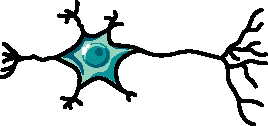
\includegraphics[width=\linewidth]{graphics/neuron}
    \caption[Schematic diagram of a neuron]{%
        Schematic diagram of a neuron.
        A typical neuron has a dendrites, a cell body, and a single axon; 
        the dendrites receive input signals from other neurons,
        and propagates output signals along the axon.
    }
    \label{fig:neuron}
\end{marginfigure}

\begin{marginfigure}%
	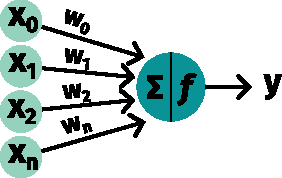
\includegraphics[width=\linewidth]{graphics/perceptron}
	\caption{Schematic diagram of a perceptron}
    \label{fig:perceptron}
\end{marginfigure}

%%%%%%%%%%%%%%%%%%%%%%%%%%%%%%%%%%%%%%%%%%%%%%%%%%%%%%%%%%%%%%%%%%%%%%%%%%%%%%%

Neural networks have been designed
using the archicteture of neurons in a human brain as inspiration.
The simplest model is that of a perceptron, 
which can be seen as a computational approximation
of a real neuron or nerve cell%
\autocite{charniakIntroduction2019}.
A typical neuron has many dendrites, a cell body, and a single axon 
(Figure~\ref{fig:neuron}).
The dendrites carries the input signal to a neuron,
and if the cumulative signal is great enough%
\sidenote{
    This threshold is known as 
    the \textit{threshold potential},
    and is typically between -50 and -55 mV.
}, 
then the neuron will propagate an action potential down the axon%
\autocite{seifterConcepts2005}.
In similar fashion, a perceptron receives may receive many different inputs
and produces a single output (Figure~\ref{fig:perceptron}).
In the case of a neuron, the \enquote{all-or-none} principle means
that nerve cells either signals at full strength or not all.
For a perceptron, this priniciple can be emulated
with the followingly step function:

\begin{equation}
    f_{\phi}(\mathbf{x})  = 
        \begin{cases}
            1 & \text{if } b + \mathbf{w} \cdot \mathbf{x} > 0\\
            0 & \text{otherwise}
        \end{cases}
\end{equation}

By combing many thousands of such neurons,
in a multilayer-perceptron or artificial neural network,
we can create a model that, 
can learn even the most complex of patterns.
Deep learning is at its core a form of representation learning.
Each layer in a neural network is a different representation,
and by stacking several of such layers on top of each others,
the representation in one hidden layer
feeds into the next layer and
is thereby being transformed into an even more abstract representation%
\autocite{estevaGuide2019}.

%%%%%%%%%%%%%%%%%%%%%%%%%%%%%%%%%%%%%%%%%%%%%%%%%%%%%%%%%%%%%%%%%%%%%%%%%%%%%%%
% insert example of abstract representations in a computervis model
%%%%%%%%%%%%%%%%%%%%%%%%%%%%%%%%%%%%%%%%%%%%%%%%%%%%%%%%%%%%%%%%%%%%%%%%%%%%%%%


\section{Regularization}

One approach to avoid overfitting in neural networks
is a technique known as dropout.
At each step of model training,
a random set of nodes in the network are disabled.
In a sense, the result is a rough approximation of 
an ensemble of different networks.


Dropout introduces noise during training
and thereby forces the network to be less senstive of noise.
Hidden units trained with dropout needs to be useful 
with or without the presence of neighboring units.

%%%%%%%%%%%%%%%%%%%%%%%%%%%%%%%%%%%%%%%%%%%%%%%%%%%%%%%%%%%%%%%%%%%%%%%%%%%%%%%

\section{Miscellaneous}

In his review on artificial intelligence in medicine%
\autocite{topolHighperformance2019}, 
Eric Topol expresses his view that in the future
\blockquote{%
almost every type of clinician, ranging from specialty doctor to paramedic,
will be using AI technology, and in particular deep learning [...]
}.

The ability to predict adverse outcomes could make  
healthcare resources more efficient.

Systematic deugging and continuous monitoring and validation 
is of utmost importance if we are to release AI algorithms into the wild%
\autocite{topolHighperformance2019}.

There has been much discussion about, and there are many opinions on, 
the black-box nature of many machine learning algorithms and 
how it should or should not affect the clinical use of such 
\autocite{topolHighperformance2019, gunningXAI2019, vanderveldenExplainable2022}.


In computer vision tasks in the medical domain,
deep-learning models have achieved physician-level performance
in many different diagnostic tasks
ranging from \todo{finish sentence}.


\chapter{Time-to-Event Prediction with Neural Networks}
\label{survival-analysis}

% marginnote {{{
\marginnote{%
    \setlength{\parindent}{0pt}
    \vskip 1em
    What is survival analysis?
    \begin{description}[leftmargin=!, labelwidth=3em]
        \item[outcome] time until an event occurs.
            Can be measured in seconds, days, months, etc.
        \item[event] death, relapse, remission, engine failure, etc.
    \end{description}
    
    \begin{center}
    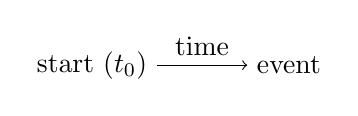
\begin{tikzpicture}
        \noindent
        \node (a) at (2.5, 0) {event};
        \node (b) at (0, 0) {start (\(t_0\))} edge ["time", ->] (a);
    \end{tikzpicture}
    \end{center}
}
% }}}

In the previous chapter, 
I gave an overview of machine learning and neural networks,
highlighting key ideas and concepts related to the studies in this thesis.
Neural networks specifically, 
were used in \studyii{} and \studyiii{} to develop
prediction models for ischemic heart disease.
These models, however, diverge from classical neural network methods.
Instead, they include modifications that make them applicable
in modelling and analysis of time-to-event data.
This chapter will provide an introduction to the fundamentals
of survival analysis and will cover the
theory that enables the implementation of such analyses with
neural network models.
% The chapter concludes with a discussion on different 
% validation methods for time-to-event prediction models.

\section{What is Survival Analysis?}

Generally, 
survival analysis is the collection of statistical methods
for the modelling and analysis of time-to-event data,
which is data where the outcome variable of interest 
is the time until \enquote{something} happens.~%
~\autocite{kleinbaumSurvival2011}
This \enquote{something} is a particular event of interest,
which, depending on the type of analytical problem, 
could be cancer relapse, 
diabetes remission,
or death.
In cardiovascular research, 
common examples of time-to-event outcomes include
\begin{enumerate*}
    \item time to death due to any cause (all-cause mortality)
    \item time to death due to a specific cause,
        e.g. sudden cardiac arrest
    \item time to first occurence of a \ac{MACE}
\end{enumerate*}.
To figure out what processes and characteristics 
that are associated with such events, 
in survival analysis, we try to model the relationship between
explanatory variables and the number of weeks, months, or years 
until that particular event is likely to occur. 

% marginnote{{{
\marginnote{%
    Survival analysis have applications outside biomedical research.
    In engineering, it is called \textit{reliability analysis} and
    is used to model the time-to-failure of system-critical components 
    such as e.g. bearings or valves.
}% }}}

Although this task can be daunting in its own right, 
an additional complication to survival analysis 
is the presence of observations that are subject to 
censoring.
This concept, censoring, refers to cases 
where the event of interest has not been observed 
before the end of follow-up, 
e.g. when a study or experiment has to be stopped.
In such cases, 
we would know that a given subject did not experience a relapse 
in the three months he or she was included in the study, 
but after the study period ends, 
we have no information on the status of the patient. 
Including and utilizing this partial information
is a cornerstone in many survival analysis problems.

There exists different forms of censoring,
such as right censoring, left censoring, and interval censoring.
In the study designs used throughout this thesis 
we have only had to deal with right censoring,
the most common form of censoring,
so the two other types will not be described further.
See instead the text book by \citeauthor{kleinSurvival2003} 
for more details on this.
~\autocite{kleinSurvival2003}

\section{Fundamentals of Survival Analysis}

In survival analysis, 
the central outcome variable is survival time,
a non-negative random variable denoted as \(T\). 
When refering to specific values of \(T\), 
a lower case \(t\) is typically used.  
A survival dataset \(\mathfrak{D}\) of size \(N\) is given by
\begin{equation}
    \mathfrak{D}_N = \{(t_i, \sigma_i, \vec{x}_i) \mid i = 1, \ldots, N\} 
\end{equation}
where \(t_i = \min(T_{i}, C_i) \) is the survival time 
for the \(i\)th subject,
with \(T_i\) denoting the survival time
and \(C_i\) denoting the censoring time. 
Also, \(\vec{x}_i = (x_1, x_2, \dots, x_p)'\) is the covariate vector
and \(\sigma_i\) is the event indicator, which is defined as
\begin{equation}
    \label{eq:sigma-def}
    \sigma_i =
        \begin{cases}
            0 & \text{if subject is censored} \; (T_i >    C_i) \\
            1 & \text{if event is observed} \; (T_i \leq C_i)
        \end{cases}
\end{equation}

In the following, I will initially be assuming that \(T\) is 
continuous and that there is an absence of competing risks, 
however both of these assumptions will later be relaxed in the discussion 
of competing risks and discrete-time survival analysis.

\subsection{Basic Survival Quantities}
\label{sub:survival-quantities}

% figure: theoretical survival function{{{
\begin{marginfigure}%
	\begin{tikzpicture}[scale=2]
	  \draw[->] (0, 0) --  (2,0) 
		node[pos=0.0, below] {$0$}
		node[pos=0.5, below] {$t$}
		node[pos=1.0, below] {$\infty$};
	  \draw[->] (0, 0) --  (0,1) 
		node[pos=1.0, left] {$1$}
		node[pos=0.5, left] {$S(t)$};
	  \draw[-, color=color2, thick] 
		(0.05, 0.95) .. controls (1, 1) and (1, 0) .. (1.90, 0.05);
	\end{tikzpicture}
    \caption[A Theoretical Survival Function]}}

In survival analysis, 
the central function of interest is 
the survival function \(S(t)\), 
that represents the probability 
of an individual still being alive after 
some specified duration of time, we have that 
%
\begin{equation}
    S(t) = \PR (T > t), \quad 0 < t < \infty.
\end{equation}

The survival function is 
the integral of the probability density function, \(f(t)\),
and is the complement to the cumulative distribution function, \(F(t)\),
which means that
~\autocite{kleinSurvival2003}
%
\begin{equation}
    S(t) = 1 - F(t) 
    \quad \text{and} \quad 
    S(t) = \int_{t}^{\infty} f(u) \, \diff u
\end{equation}

Another fundamental quantity is the hazard function, or hazard rate,
which represents the instantaneous failure rate at a given timepoint,
and is defined as
%
\begin{equation}
    \label{eq:hazard-function}
    \lambda(t) = \lim_{\Delta t \to 0} 
        \frac{\PR (t \leq T < t + \Delta t \mid T \geq t)}{\Delta t}
\end{equation}
% 
from which it can be shown that
~\autocite{kleinSurvival2003}
%
\begin{equation}
    \lambda(t) = \frac{f(t)}{S(t)} = -\frac{\diff}{\diff t} \ln[S(t)].
\end{equation}
%
and thus the hazard function completely describes the distribution of \(T\),
such that all the the other quantities can be obtained from it---%
as well as the other way around.

In terms of its interpretation, 
from \cref{eq:hazard-function} it follows that \(\lambda(t)\Delta t\) 
is a measure of the conditional probability of failure in a small time
window, given that the individual is still alive at time \(t\).
~\autocite{kleinSurvival2003}

Analogous to the relation between \(f(t)\) and \(F(t)\), 
integrating \(\lambda(t)\) with resport to \(t\),
we obtain cumulative hazard function, defined as
%
\begin{equation}
    \Lambda(t) = \int_{0}^{t} \lambda(u) \, \diff u = -\ln[S(t)].
\end{equation}

\subsection{The Kaplan-Meier Estimator}

The survival function of a population,
can be estimated using the Kaplan-Meier method,
which is the standard estimator of the survival function.
~\autocite{kaplan1958nonparametric}
~\autocite{kleinSurvival2003}
In this approach, 
the distinct failure times are ordered such that%
\footnotemark
\begin{equation*}
    t_{(1)} < t_{(2)} < \ldots < t_{(j)},
\end{equation*}
%
and we introduce two quantities to keep track of
the number of failures \(\widebar{D}(j)\), 
as well as the number of subjects still at risk \(\widebar{A}(j)\).
They are defined as
\begin{equation}
\begin{aligned}
    \bar{D}(j) &= \card \{i \in \{1, \dots, n\} \mid t_i = t_{(j)}, \sigma_i = 1\} \\
    \bar{A}(j) &= \card \{i \in \{1, \dots, n\} \mid t_i > t_{(j)}\},
\end{aligned}
\end{equation}
and the Kaplan-Meier estimator can then be formulated as 
\begin{equation}
    \widehat{S}(t)
    =   \prod_{j \mid t_{(j)} \leq t} 
        \frac{
            \bar{A}(j) -
            \bar{D}(j)
        }{
            \bar{A}(j)
        }
    =   \prod_{j \mid t_{(j)} \leq t} 
        1 - \frac{
            \bar{D}(j)
        }{
            \bar{A}(j)
        }.
\end{equation}

\footnotetext{%
    Following the example of [\cite{kleinbaumSurvival2011}], 
    the \(t\)'s denoted with subscripts within parentheses \(t_{(j)}\)
    refers to the \(j\)th element of the ordered distinct failure times and
    are thus different from \(t_1, t_2, \ldots, t_i\) that refers to the 
    observed failure time of subject \(1\), \(2\), and \(i\)
}

The Kaplan-Meier estimator is thus as step-function that decreases
after each observed event.
While the Kaplan-Meier estimator is useful 
for summarising the survival of a population, 
it does not account for the effect of covariates.
Instead, another approach is needed for regression analyses.

\subsection{Cox's Proportional Hazards Model}

To describe and model the relationship between explanatory variables
and time-to-event phenomenons, a widely used statistical model is 
the Cox proportional hazards model. 
~\autocite{coxRegression1972}
This model seeks to model the hazard function over time \(t\),
of an individual with a covariate vector \(\vec{x} = (x_1, x_2, \dots)'\),
and assumes that it takes the form of
%
\begin{equation}
    \label{eq:cox}
    \widehat{\lambda} (t \,|\, \vec{x}) = \hzt \exp [g(\vec{x})],
\end{equation}
%
where \(\hzt\)
is an unspecified baseline hazard function,
and \(g(\vec{x})\) is some parametric function.
For this reason, the Cox model 
is referred to as a semi-parametric model.
In its classical formulation, 
this function is a linear combination of parameters 
\(\vec{\beta}\) and covariates \(\vec{x}\),
as given by

\begin{equation}
    g(\vec{x}) 
    = \vec{\beta}' \vec{x} 
    = \beta_1 x_1 + \beta_2 x_2 + \ldots + \beta_p x_p
\end{equation}

In estimation of the parameters \(\vec{\beta}\),
the baseline hazard \(\hzt\) is treated as a nuisance function
and the coefficients are estimated by
maximising a partial likelihood
in which \(\hzt\) has been abstracted away.
~\autocite{kalbfleischStatistical2002}

A central assumption in the Cox model, 
at least in the standard version with fixed covariates
(\(\vec{\beta}\) instead of \(\vec{\beta}(t)\)),
is that of proportional hazards.
Let \(\vec{x}\) and \(\vec{x}'\) be two different 
covariate vectors, now the ratio between their
respective Cox-estimated hazards is

\begin{equation}
    \label{eq:hazard-ratio}
    \begin{aligned}
    \frac%
        {\widehat{\lambda}(t \,|\, \vec{x} \hfill)}%
        {\widehat{\lambda}(t \,|\, \vec{x'})}
    &=
    \frac%
        {\hzt \exp (\vec{\beta}\cdot\vec{x}\hfill)}%
        {\hzt \exp (\vec{\beta}\cdot\vec{x'})} \\
    &=
    \frac%
        {\exp (\vec{\beta}\cdot\vec{x}\hfill)}%
        {\exp (\vec{\beta}\cdot\vec{x'})} \\
    &= \exp (\vec{\beta} \cdot (\vec{x} - \vec{x'}))
    \end{aligned}
\end{equation}

Since the right-hand side of the equation does not include a term for \(t\),
the hazard ratio between the two samples are constant and 
they are thus proportional to one another., 
This shows that by assuming the hazard takes the form of \cref{eq:cox},
then it is also assumed that the hazards between two subjects are proportional.
Although this assumption is a strong one, 
and the validity of the Cox model relies on it, 
the assumption makes interpretation of parameters easier.
~\autocite{tutzModeling2016}
For example, 
in an randomized clinical trial
studying the survival effect of a new type of medication, 
we can let \(x = 1\) represent the experimental treatment  
and \(x' = 0\) represent standard of care, 
then the hazard ratio in \cref{eq:hazard-ratio} takes the form of
%
\begin{equation}
      \exp \left(\beta (x - x')\right)
    = \exp \left(\beta (1 - 0)\right)
    = \exp (\beta ),
\end{equation}
%
which means that if \(\beta < 0\), 
then the hazard of the experimental treatment is 
\(\exp({\beta})\) times lower than standard of care
and should therefore be preferred.%
\sidenote{% 
This example is a slightly modified version of the 
one given in \cite[pp. 50]{tutzModeling2016}}


\section{Analysis of Competing Risks}

\begin{marginfigure}[3em]% {{{
    \tikzstyle{outcome}=[%
        rectangle, rounded corners, minimum height=5mm, fill=color3
    ]
    \centering
    \begin{tikzpicture}[x=0.60\linewidth, y=1cm]
    \graph [edge quotes={font=\scriptsize, fill=white}, 
            nodes      ={draw, outcome, sloped, minimum width=1cm}]{
        alive [fill=color4] -> dead [> "\(\lambda(t)\)" ];
    };
    \end{tikzpicture}
    \caption[A Single State Model]{
        A simple survival analysis setup 
        involves modelling a single transition between states 
        \enquote{alive} and \enquote{dead}.
    }
    \label{fig:ssm}
\end{marginfigure}% }}}

Up to this point, the description of concepts in survival analysis has
assumed the presence of only a single event type, such as all-cause mortality
(\cref{fig:ssm}).
In practice, particularly in clinical settings, 
this single-event model can be too restrictive,
and instead one needs to consider competing risks
(\cref{fig:msm}).
By definition, a competing risk is a secondary event whose occurence 
prevents the primary event from occuring.
For example,
in a study where the primary outcome is cardiovascular mortality,
deaths from non-cardiovascular causes are a competing risk.

In the following, 
we let \(R \in \{1, \dots, \kappa\}\) denote the \(\kappa\) different competing risks,
and then slightly update the definition of the event indicator \(\sigma_i\)
(\cref{eq:sigma-def}), such that
\begin{equation}
    \label{eq:sigma-def-2}
    \sigma_i =
        \begin{cases}
            0 & \text{if subject is censored} \; (T_i >    C_i) \\
            r & \text{if cause r is observed} \; (T_i \leq C_i, R = r).
        \end{cases}
\end{equation}

\begin{marginfigure}% {{{
    \tikzstyle{outcome}=[%
        rectangle, rounded corners, minimum height=5mm, fill=color3
    ]
    \centering
    \begin{tikzpicture}[x=0.60\linewidth, y=0.85cm]
    \graph [edge quotes={font=\scriptsize, fill=white}, 
            nodes      ={draw, outcome, sloped, minimum width=1cm}]{
        alive [fill=color4] -> {
            cause 1 [> "\(\lambda_1(t)\)" ],
            cause 2 [> "\(\lambda_2(t)\)" ],
            cause k [> "\(\lambda_\kappa(t)\)" ],
        };
    };
    \end{tikzpicture}
    \caption[A Multi-State Model]{
        A survival analysis setup with competing risks
        involves modelling transitions between states 
        \enquote{alive} and \(k\) different absorbing
        states, \enquote{cause 1} to \enquote{cause \(\kappa\)}
    }
    \label{fig:msm}
\end{marginfigure}
% }}}

\subsection{Cause-Specific Survival Quantities}

To describe time-to-event phenomena with competing risks, 
we introduce the cause-specific hazard function and 
cumulative-incidence function.
With \(R \in \{1, \dots, \kappa\}\) denoting the \(\kappa\) different competing risks, 
the cause-specific hazard function is defined as
\begin{equation}
    \lambda_r(t) = \lim_{\Delta t \to 0} 
        \frac{\PR (t \leq T < t + \Delta t, R=r \mid T \geq t)}{\Delta t}
\end{equation}
where \(r\) refers to a specific value of \(R\).
The cause-specific cumulative incidence function is defined as
~\autocite{kalbfleischStatistical2002}
\begin{equation}
    F_r(t) = \PR(T \leq t, R = r).
\end{equation}

The overall hazard and cumulative incidence, 
which combines failures of any of the \(\kappa\) causes,
correspond to the hazard function 
and the cumulative distribution function 
in the single-event setting, that is
\begin{equation}
    \lambda(t) = \sum_{r=1}^{\kappa} \lambda_r(t)
    \quad \text{and} \quad
    F(t) = \sum_{r=1}^{\kappa} F_r(t).
\end{equation}

\subsection{The Aalen-Johansen Estimator}

In the competing risk setting, 
some of the methodology previously presented
have to be slightly adjusted.
For example, 
simply treating competing events as censored 
and applying the standard Kaplan-Meier estimator, 
would lead to a biased estimate of \(F(t)\).
~\autocite{pepeKaplan1993}
Instead, an alternative approach is the Aalen-Johansen estimator
that allows estimation of the cause-specific cumulative incidence.
~\autocite{aalenEmpirical1978}
Of note, the Aalen-Johansen is a general method for estimating
transition probabilities in state-transition models,
and can be used to describe complex multi-state models,
including those with repeated events and with non-terminal states.
~\autocite{survival-package}
However, we will be assuming a standard competing-risk setting
with \(\kappa\) different terminal states, 
as depicted in \cref{fig:msm}.
 
If we again order the distinct failure times, 
corresponding to any cause, 
such that
\(t_{(1)} < t_{(2)} < \ldots < t_{(j)}\),
and update the definition of \(\bar{D}(j)\) to keep track of cause-specific
events, such that we have
\begin{equation}
\begin{aligned}
    \bar{D}(j, r) &= \card \{i \in \{1, \dots, n\} \mid t_i = t_{(j)}, r_i = r\} \\
    \bar{A}(j)    &= \card \{i \in \{1, \dots, n\} \mid t_i > t_{(j)}\}.
\end{aligned}
\end{equation}
Now, the Aalen-Johansen estimator of the cumulative incidence function
can be defined as 

\begin{equation}
    \widehat{F}_r(t)
    =   \sum_{j \mid t_{(j)} \leq t}{
        \!\!
        \widehat{S}(t_{(j-1)})
        \frac{\bar{D}(j, r)}{\bar{A}(j)}
    }
\end{equation}

\section{Time-to-Event Prediction}

Up until now, 
I have outlined various concepts foundational to survival analysis,
focusing primarily on quantities and statistics of time-to-event outcomes
at a popoulation level.
These measures play an important role in understanding 
and interpretation of survival data.

In the context of precision medicine, however,
the emphasis shifts towards making individualized predictions
taking distinct patient-level characteristics into account.
Consequently, as described in \cref{chap:ml-and-nn}, 
the primary concern lies in 
making accurate predictions on unseen data,
rather than in the exploration of disease etiology and underlying mechanisms.

For prediction of time-to-event outcomes, classical approaches 
include models based on the previously presented semi-parametric Cox model 
as well as various parametric survival models, 
such as those based on exponential, Weibull, or log-normal distributions.
~\autocite{kleinSurvival2003}
This thesis, however, 
explores the use of contemporary machine learning methods 
in time-to-event prediction,
with a particular emphasis on the application of neural networks.

\subsection{Neural Networks and Time-to-Event Outcomes}

The first application of neural networks for time-to-event prediction
was demonstrated by
\citeauthor{faraggiNeural1995} in
\citeyear{faraggiNeural1995},
and involves parameterising the parametric part of the Cox model
with a neural network, 
such that the \(g(\vec{x})\) term in \cref{eq:cox} is a 
flexible neural network model instead of a simple linear function.
\autocite{faraggiNeural1995}

\vspace{.5em}
\begin{equation*}
    \widehat{\lambda} (t \,|\, \vec{x}) = \hzt \exp [
    \eqnmarkbox[color2]{node1}{
        g(\vec{x})
    }]
\end{equation*}
\annotate[yshift=.6em]{left}{node1}{use neural network}

This approach was later further refined
in the \emph{DeepSurv} paper from 
\citeyear{katzmanDeepSurv2018a},
in which modern neural network techniques
were added to Faraggi-Simon framework, 
which markedly improved its usefulness.
~\autocite{katzmanDeepSurv2018a}
\citeauthor{katzmanDeepSurv2018a} showed that the flexibility 
offered by neural networks led to increased performance
in both synthetic and real-life time-to-event prediction applications
compared to a standard Cox model.
However, the \emph{DeepSurv} approach is still limited by the 
assumption of proportional hazards.

\subsection{Overview of Approaches}

Recently, there have been considerable interest in neural network-based
time-to-event prediction models, and as a consequence, many new methods 
have since been developed.
For a thorough overview of the existing approaches, 
\textcite{wiegrebeDeep2023} and 
\textcite{kvammeContinuous2021} provide valuable insights.
Generally, two prevailing types of approaches exists:
continuous-time methods based on the Cox model, 
which includes \emph{DeepSurv},
and discrete-time methods as exemplified by 
\textcite{leeDeepHit2018} and \textcite{gensheimerScalable2019}.

The discrete-time approaches offer several advantages that 
make them particularly relevant for neural network. 
Furthermore, they have been shown to offer better predictive
performance compared to the Cox-based methods.
~\autocite{kvammeContinuous2021, leeDeepHit2018, gensheimerScalable2019}
Notably, \emph{DeepHit}\autocite{leeDeepHit2018}
and \emph{Logistic-Hazard}\autocite{gensheimerScalable2019}
are the two most cited papers in this context as of the time of writing.
Among these and other tested approaches,
\textcite{kvammeContinuous2021} found that 
DeepHit offers excellent discrimination but suffers from poor calibration.
In contrast, the Logistic-Hazard model have nearly as good discrimination
and also significantly better calibration. 
Consequently, the Logistic-Hazard model, and an extension hereof, 
was chosen for application in 
\studyii{} and \studyiii{}.

In the following section, I will be giving a brief description of
this discrete-time formulation of time-to-event analysis and 
elaborate on the Logistic-Hazard model in more detail.

\section{Discrete-Time Survival Analysis}

Most textbooks on survival analysis treats survival time as continuous, 
and that is also usually the case across the biomedical litterature.
However, handling time as a something discrete can be advantegous.
In practice, most measurements of time is inherently discrete 
with durations being recorded in, for example, days; months; and weeks.
The continuous time approaches presented earlier in this chapter, 
are also applicable to discrete time data,
however, methods designed specifically for discrete time-to-event 
data have some advantages~\autocite{tutzModeling2016}:

\begin{itemize}
    \item If observed event times are inherently discrete, 
        then modelling them as such is arguably more appropriate. 
    \item In the discrete-time setting, hazards can be formulated as 
        conditional probabilities which are much more intuitive to 
        both interpret and understand.
    \item Discrete time-to-event models are more easily transferred to 
        other more general purpose modelling frameworks 
        such as generalized linear models, random survival forests, 
        neural networks.
\end{itemize}

The latter point is the main motivation behind both 
the \emph{DeepHit} and \emph{Logistic-Hazard} approach.
For a complete overview of the theory enabling these two approaches,
the book by \textcite{tutzModeling2016} is a valuable resource, 
and serves as the main source of reference for the following.

\subsection{Notation and Definitions}

In the discrete-time framework, 
continuous follow-up time \(\Tic\) is divided into \(q\) contiguous intervals,
that is
%
\begin{equation*}
	(0, a_1], (a_1, a_2], \dots, (a_{q-1}, a_q]
\end{equation*}
%
and \(\Tid \in \{1, \dots, q\}\) is a discrete random  variable
such that if \(\Tid = \tid\) is observed, then the event 
falls in the interval \((a_{\tid-1}, a_{\tid}]\).
Similarly, the discretized censoring time is \(\Cid \in \{1, \dots, q\}\).

With this discrete time scale, 
the distribution of \(\Tid\), 
given some vector of covariates \(\vec{x}\),
can be described using discrete equivalents of the previously 
outlined basic quantities of survival analysis, that is
%
\begin{align}
    \text{probability mass function:} \qquad
    f(\tid \giv \vec{x}) 
    &= \PR (\Tid = \tid \mid \vec{x}) \\
    %
    \text{cumulative mass function:} \qquad
    F(\tid \giv \vec{x}) 
    &= \PR (\Tid \leq \tid \mid \vec{x}) \\
    %
    \label{eq:discrete-hazard}
    \text{hazard function:} \qquad
    \lambda(\tid \giv \vec{x}) 
    &= \PR (\Tid = \tid \mid \Tid \geq \tid, \vec{x}) \\
    %
    \text{survival function:} \qquad
    S(\tid \giv \vec{x}) 
    &= \PR (\Tid > \tid \mid \vec{x})
\end{align}

\subsection{The Logistic-Hazard Model}

\Citeauthor{gensheimerScalable2019}'s approach, 
which they refer to as \enquote{Nnet-survival},
~\autocite{gensheimerScalable2019}
is more accurately characterized as the Logistic-Hazard method, 
as described in \textcite{kvammeContinuous2021}.
In the Logistic-Hazard method, 
the time-to-event data is described by 
modelling the effect of covariates on the discrete hazard function 
(\cref{eq:discrete-hazard}) 
using a neural network.
The concept is not novel, 
employing the discrete hazard for statistical modeling is a common method, 
as covered extensively in \textcite{tutzModeling2016}. 
In addition, a neural-network based model with the same general idea 
was presented by \citeauthor{brownUse1997} in 1997.
~\autocite{brownUse1997}
However, 
\citeauthor{gensheimerScalable2019} were the first to adapt the approach
to current neural network methodologies.

\subsection{Log-Likelihood of the Discrete Hazard}

Let \(\mathfrak{D}_{\mathrm{d}}\) 
be a discrete-time survival dataset of size \(N\),
\begin{equation}
    \mathfrak{D}_{\mathrm{d}} = 
    \{(\tid_i, \sigma_i, \vec{x}_i) \mid i = 1, \ldots, N\},
\end{equation}
where \(\tid_i\) is the discretized survival time, 
\(\sigma_i\) is the event indicator as defined in \cref{eq:sigma-def},
and \(\vec{x}_i = (x_1, x_2, \dots, x_p)'\) is the feature vector.
With the assumption of \emph{noninformative censoring},
~\autocite{kalbfleischStatistical2002}
in the Logistic-Hazard model, 
the contribution of the \(i\)th individual to the likelihood function
can be shown to be  
~\autocite{tutzModeling2016}
\begin{equation}
    \Lik_i = %
    \begin{cases}
        \PR (\Tid_i = \tid_i) & \text{if non-censored} \\
        \PR (\Tid_i > \tid_i) & \text{if censored}.
    \end{cases}
\end{equation}

These two probabilities can be expressed using the discrete hazards,
as it can be seen that
\begin{align}
    \begin{split}
    \PR (\Tid = \tid) 
    &= \PR (\Tid = \tid \mid \Tid \geq \tid) \PR (\Tid  \geq \tid) \\
    &= \PR (\Tid = \tid \mid \Tid \geq \tid) \PR (\Tid  > \tid - 1) \\
    &= \lambda (\tid) \, \prod_{s=1}^{\tid - 1} (1 - \lambda(s))
    \end{split} \\
    \intertext{and similarly}
    \begin{split}
    \PR (\Tid > \tid) 
        &= \PR (\Tid > \tid \mid \Tid \geq \tid) \PR (\Tid  \geq \tid) \\
        &= (1 - \PR (\Tid = \tid \mid \Tid \geq \tid)) \PR (\Tid  \geq \tid) \\
        &= (1 - \PR (\Tid = \tid \mid \Tid \geq \tid)) \PR (\Tid  > \tid - 1) \\
        &= \prod_{s=1}^{\tid} (1 - \lambda(i)).
    \end{split}
\end{align}

Now, by introducing an indicator function, 
defined according to \textcite{tutzModeling2016} as 
\begin{equation}
    \label{eq:lh-indicator}
    \bar{y}_i(\tid) = \begin{cases}
        1, & \text{if individual fails in \((a_{\tid-1}, a_{\tid}]\),} \\
        0, & \text{if individual survives \((a_{\tid-1}, a_{\tid}]\),}
    \end{cases}
\end{equation}
and by including the discrete hazard function and the covariates, 
the likelihood contribution for the \(i\)th individual can be expressed as
\begin{equation}
    \label{eq:lh-likelihood}
    \Lik_i = \prod_{s=1}^{\tid_i} 
        \lambda(s \giv \vec{x}_i)^{\bar{y}_i(s)}
        (1 - \lambda(s \giv \vec{x}_i))^{1 - \bar{y}_i(s)}.
\end{equation}

The total log-likelihood of all datapoints then gives the loss-function
used in the Logistic-Hazard model, 
~\autocite{gensheimerScalable2019, tutzModeling2016}
which can be expressed
\begin{equation}
    \label{eq:lh-loglikelihood}
    \lik = 
        \sum_{i = 1}^{N} 
            \sum_{s=1}^{\tid_i} 
                \bar{y}_i(s) \log (\lambda(s\giv\vec{x}_i))
                + (1 - \bar{y}_i(s)) \log (1 - \lambda(s\giv\vec{x}_i)).
\end{equation}

\subsection{Loss Function Explained}

\def\y#1#2{\hat{\lambda}_{#1#2}}
\def\yy#1#2{1\!-\!\y{#1}{#2}}

As an example, the following set of observations with discretized 
time-to-event data with a single risk, e.g. all-cause mortality, 
and a follow-up time that have been discretized into seven contiguous intervals,
constitutes a survival dataset.

\begin{equation}
\begin{tabular}{r  ccccc}
    \toprule
    subject   \(i\)      & 1 & 2 & 3 & 4 & 5 \\
    \midrule
    time    \(\tau_i\)   & 5 & 7 & 4 & 5 & 3 \\
    event   \(\sigma_i\) & 1 & 1 & 0 & 0 & 1 \\
    \bottomrule
\end{tabular}
\end{equation}

In this setting,  using the Logistic-Hazard model, 
the neural network output for this dataset is a 2-dimensional
matrix with \(5\) rows  (subjects) and \(7\) columns (time intervals),
and each entry is the predicted conditional hazard for the
specific subject at a specific timepoint. We can write this as
\begin{equation}
\hat{\bm{\Lambda}}= \!\!\!\!
\begin{tikzpicture}
[   on grid,
    font = \small,
    baseline = -.7ex,
    inner sep=1pt,
    outer sep=0pt,
    minimum width=9mm,
    minimum height=6mm,
    every left delimiter/.style={xshift=2.5ex},
    every right delimiter/.style={xshift=-3.0ex}
]
\matrix (pred) [
	matrix of math nodes, 
    left delimiter={[}, 
    right delimiter={]},
]{ 
\y{1}{1} & \y{1}{2} & \y{1}{3} & \y{1}{4} & \y{1}{5} & \y{1}{6} & \y{1}{7} \\
\y{2}{1} & \y{2}{2} & \y{2}{3} & \y{2}{4} & \y{2}{5} & \y{2}{6} & \y{2}{7} \\
\y{3}{1} & \y{3}{2} & \y{3}{3} & \y{3}{4} & \y{3}{5} & \y{3}{6} & \y{3}{7} \\
\y{4}{1} & \y{4}{2} & \y{4}{3} & \y{4}{4} & \y{4}{5} & \y{4}{6} & \y{4}{7} \\
\y{5}{1} & \y{5}{2} & \y{5}{3} & \y{5}{4} & \y{5}{5} & \y{5}{6} & \y{5}{7} \\
};
\useasboundingbox[anchor=center] (pred.north west) rectangle (pred.south east);
\draw[->, black!50] ([xshift=2ex] pred-1-7.north east) -- ([xshift=2ex] pred-2-7.east)
    node [midway, font=\scriptsize, above, sloped] {subject};
\draw[->, black!50] ([yshift=1ex] pred-1-6.north) -- ([yshift=1ex] pred-1-7.north)
    node [midway, font=\scriptsize, above] {time};
\end{tikzpicture}
\end{equation}

Now, the indicator function can be computed 
using the defintion in \cref{eq:lh-indicator}
and the observed data \(\tid_i\) and \(\sigma_i\). 
In matrix form, the output of this function is
\begin{equation}
\bar{\bm{Y}}= \!\!\!\!
\begin{tikzpicture}
[   on grid,
    font = \small,
    baseline = -.7ex,
    inner sep=1pt,
    outer sep=0pt,
    minimum width=9mm,
    minimum height=6mm,
    every left delimiter/.style={xshift=2.5ex},
    every right delimiter/.style={xshift=-3.0ex}
]

\matrix (mask) [
	matrix of math nodes, 
    left delimiter={[}, 
    right delimiter={]}
]{ 
0 & 0 & 0 & 0 & 1 & - & - \\
0 & 0 & 0 & 0 & 0 & 0 & 1 \\
0 & 0 & 0 & 0 & - & - & - \\
0 & 0 & 0 & 0 & 0 & - & - \\
0 & 0 & 1 & - & - & - & - \\
};
\useasboundingbox[anchor=center] (mask.north west) rectangle (mask.south east);
\end{tikzpicture}
\end{equation}

Now, combining these two matrices according to the formula
in \cref{eq:lh-likelihood}, we obtain the likelihood in matrix form as
\begin{equation}
    \mathcal{L}(\bm{\hat{\Lambda}}, \bm{\bar{Y}}) = \!\!\!\!
\begin{tikzpicture}
[   on grid,
    font = \small,
    baseline = -.7ex,
    inner sep=1pt,
    outer sep=0pt,
    minimum width=9mm,
    minimum height=6mm,
    every left delimiter/.style={xshift=2.5ex},
    every right delimiter/.style={xshift=-3.0ex}
]
\matrix (loss) [
	matrix of math nodes, 
    left delimiter={[}, 
    right delimiter={]},
    nodes={font=\footnotesize}
]{ 
\yy{1}{1} & \yy{1}{2} & \yy{1}{3} & \yy{1}{4} & \y{1}{5}  & -         & -         \\
\yy{2}{1} & \yy{2}{2} & \yy{2}{3} & \yy{2}{4} & \yy{2}{5} & \yy{2}{6} &  \y{2}{7} \\
\yy{3}{1} & \yy{3}{2} & \yy{3}{3} & \yy{3}{4} & -         & -         & -         \\
\yy{4}{1} & \yy{4}{2} & \yy{4}{3} & \yy{4}{4} & \yy{4}{5} & -         & -         \\
\yy{5}{1} & \yy{5}{2} & \y{5}{3}  & -         & -         & -         & -         \\
};
\useasboundingbox[anchor=center] (loss.north west) rectangle (loss.south east);
\end{tikzpicture}
\end{equation}
from which the log-likelihood, \cref{eq:lh-loglikelihood}, is then
\begin{equation*}
    \small
\begin{split}
    \mathscr{l}(\bm{\hat{\Lambda}}, \bm{\bar{Y}})
    &={} \log (\yy{1}{1}) + \log(\yy{1}{2}) + \log(\yy{1}{3}) + \log(\yy{1}{4}) 
     +  \log(\y{1}{5}) \\ 
    &+{} \log (\yy{2}{1}) + \log(\yy{2}{2}) + \log(\yy{2}{3}) + \log(\yy{2}{4}) 
     +  \log(\yy{2}{5}) + \log(\yy{2}{6}) +  \log(\y{2}{7}) \\
    &+{} \log (\yy{3}{1}) + \log(\yy{3}{2}) + \log(\yy{3}{3}) + \log(\yy{3}{4}) \\
    &+{} \log (\yy{4}{1}) + \log(\yy{4}{2}) + \log(\yy{4}{3}) + \log(\yy{4}{4}) 
    + \log(\yy{4}{5})  \\
    &+{} \log (\yy{5}{1}) + \log(\yy{5}{2}) + \log(\y{5}{3} )
\end{split}
\end{equation*}


\chapter*{Misc}

A specific chromosomal translocation in 
chronic myeloid leukemia (CML) 
results in a constitutively active tyrosine-kinase (BCR-ABL)
that can be targeted with tyrosine kinase inhibitors such as imatinib~%
\autocite{drukerEfficacy2001}.




\chapter{Results of Manuscripts}
\label{results}

\chapter{Conclusions and Future Perspectives}
\label{conclusions}

\section{Topics to be discussed}
\begin{itemize}
    \item Consider doing ablation studies to produce less-complex versions
        of the predictions models.
    \item Lack of prospective validation of medical prediction models
    \item Lack of clinical deployment and adoption 
    \item Limitations of explainable AI
\end{itemize}




%%%%%%%%%%%%%%%%%%%%%%%%%%%%%%%%%%%%%%%%%%%%%%%%%%%%%%%%%%%%%%%%%%%%%%%%%%%%%%%

\backmatter

\addcontentsline{toc}{chapter}{List of References}
\printbibliography

%%%%%%%%%%%%%%%%%%%%%%%%%%%%%%%%%%%%%%%%%%%%%%%%%%%%%%%%%%%%%%%%%%%%%%%%%%%%%%%

\appendix

\addcontentsline{toc}{chapter}{Appendix A: Manuscript I, II, and III}
% \part*{Paper 1}
% \addcontentsline{toc}{chapter}{Paper 1}
% 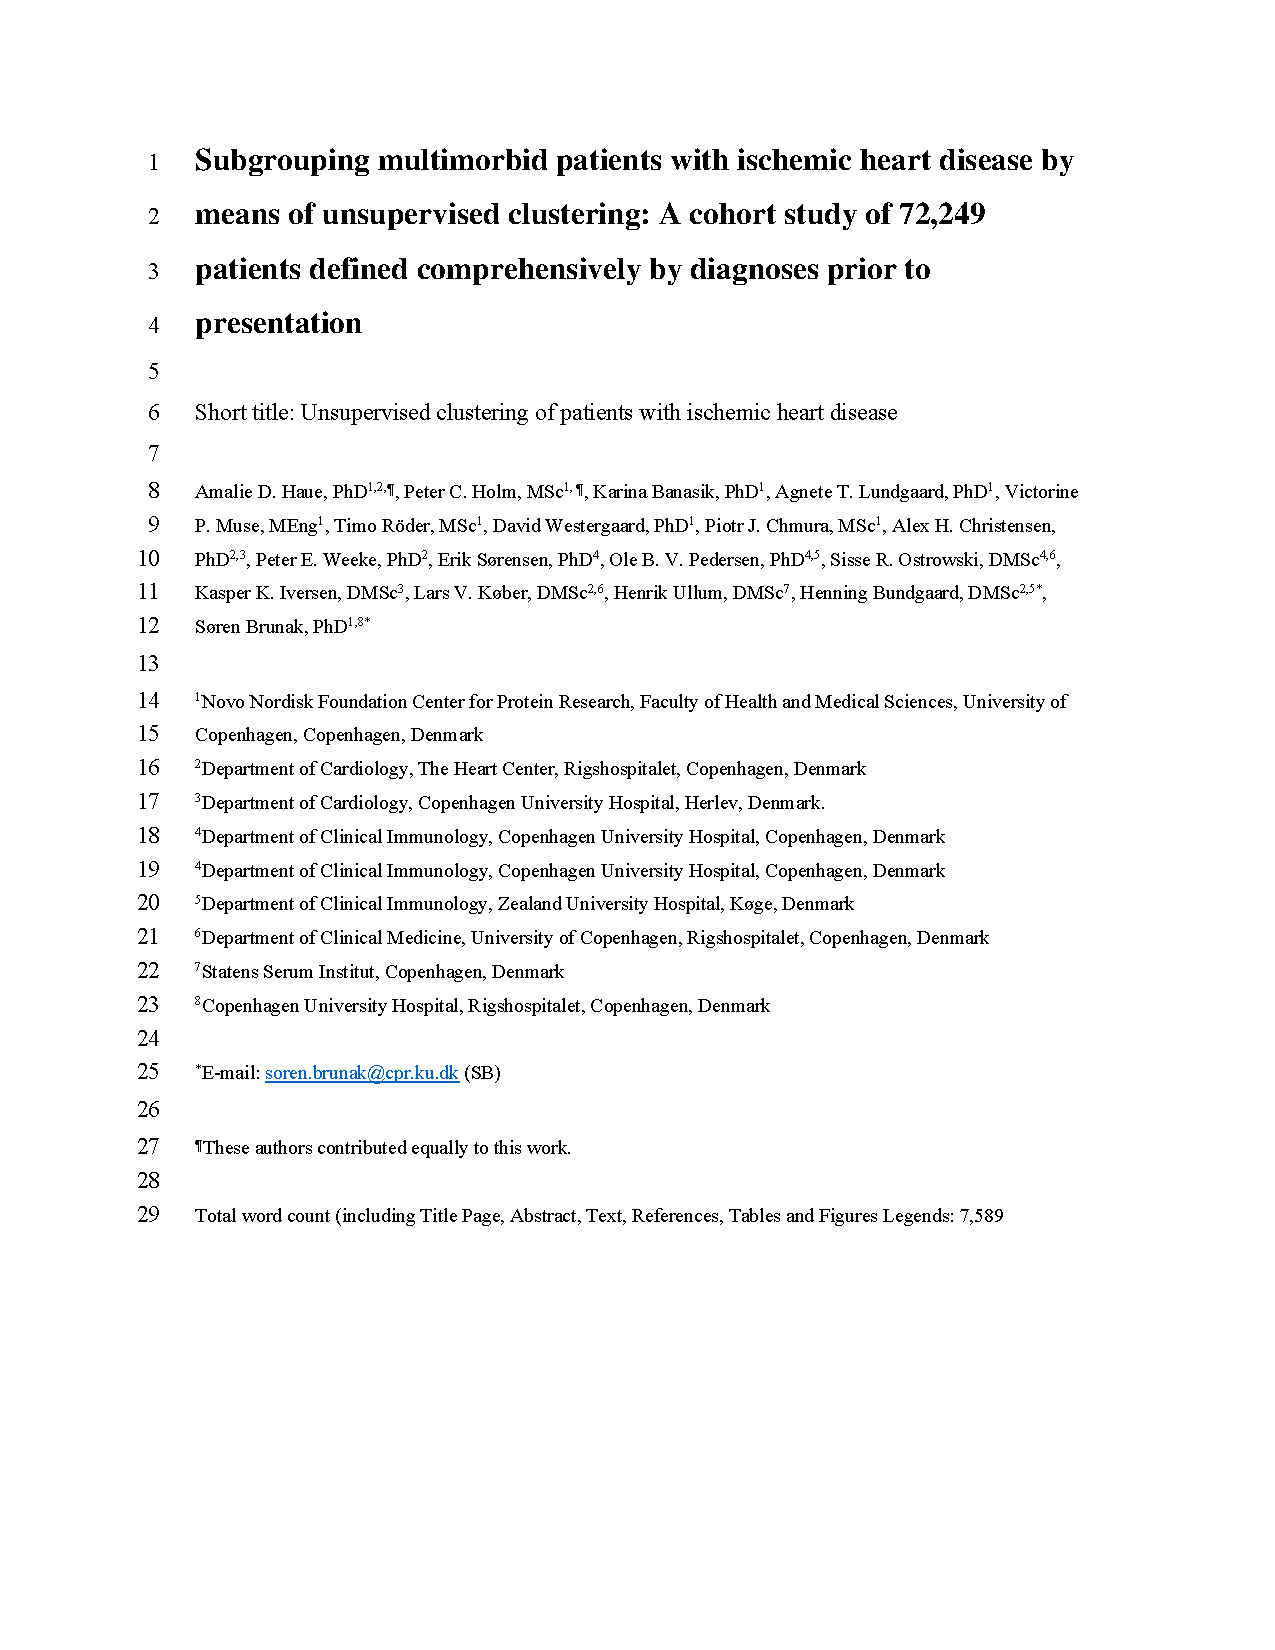
\includepdf[%
%     frame=true, scale=0.8, pages=-, pagecommand={}%
% ]{assets/paper1-clustering.pdf}
% 
% \part*{Paper 2}
% \addcontentsline{toc}{chapter}{Paper 2}
% 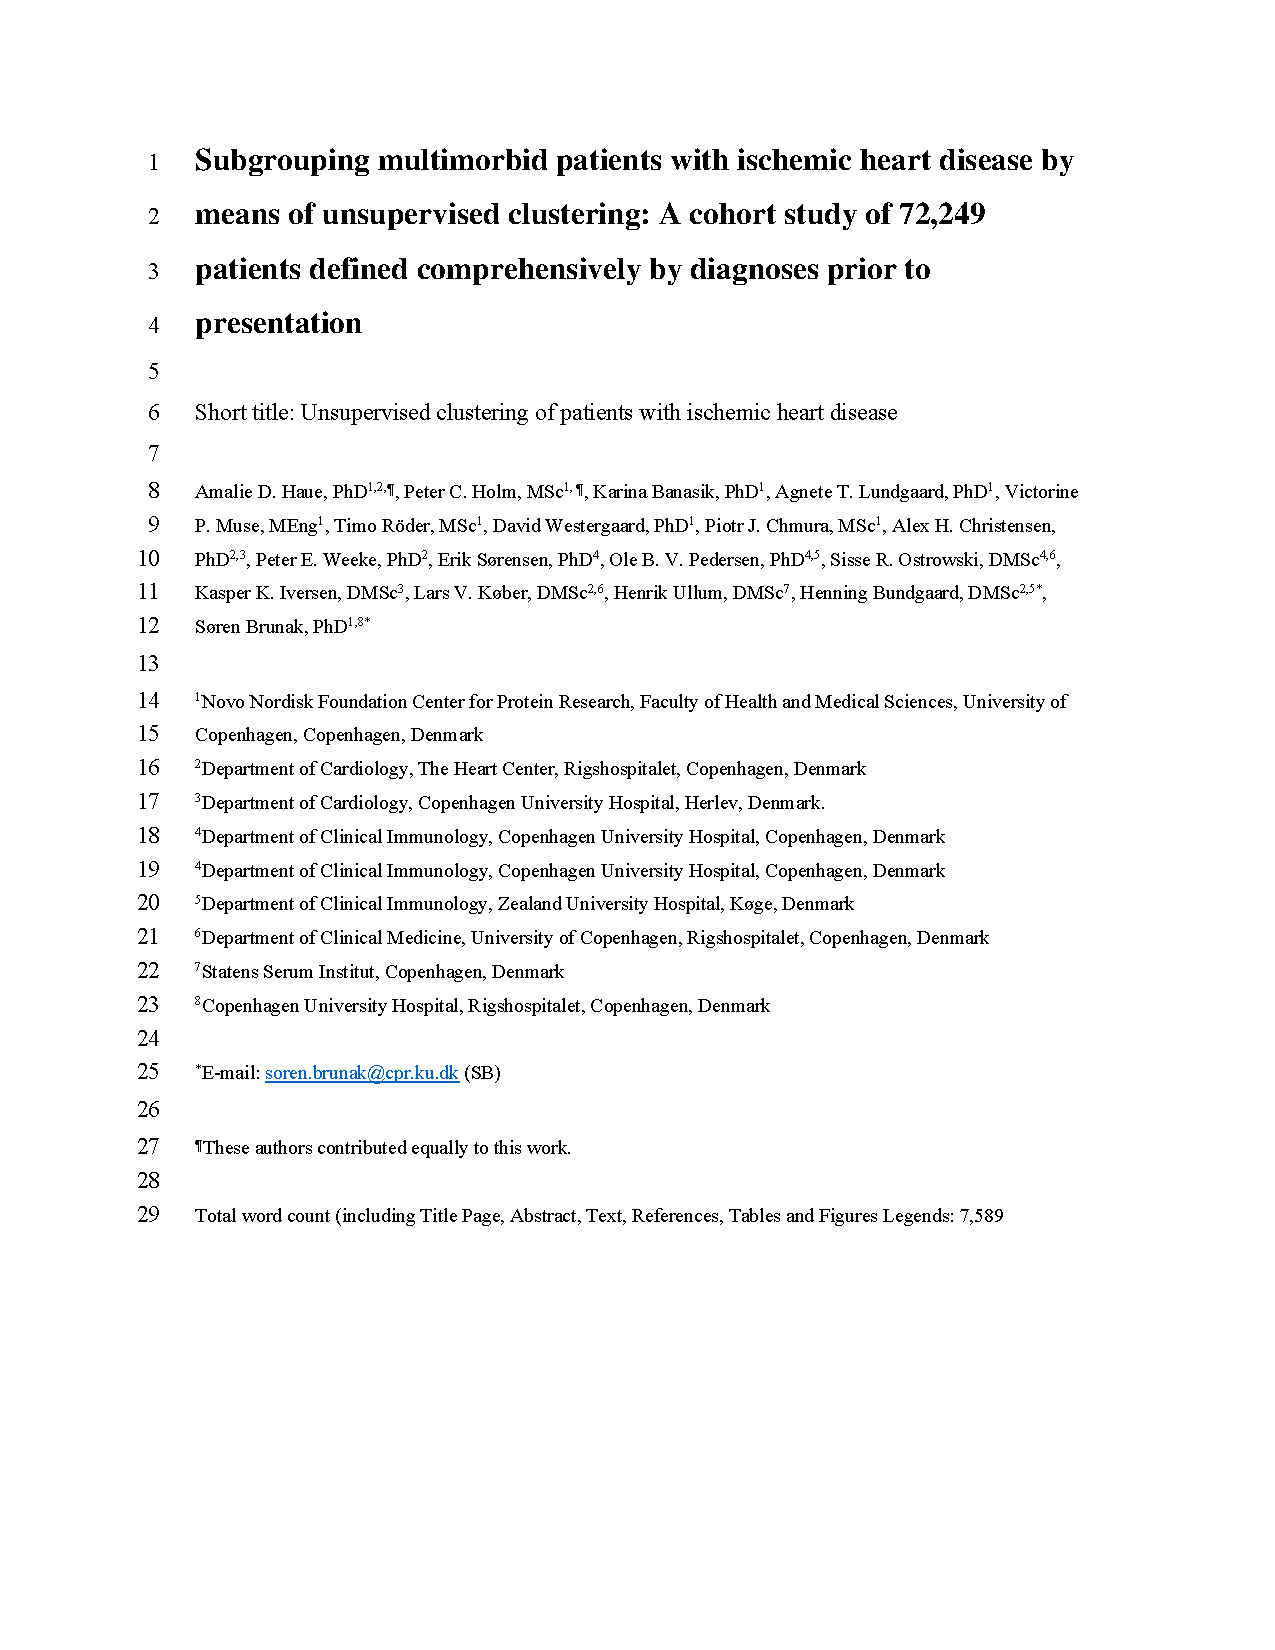
\includepdf[%
%     frame=true, scale=0.8, pages=-, pagecommand={}%
% ]{assets/paper1-clustering.pdf}
% 
% \part*{Paper 3}
% \addcontentsline{toc}{chapter}{Paper 3}
% 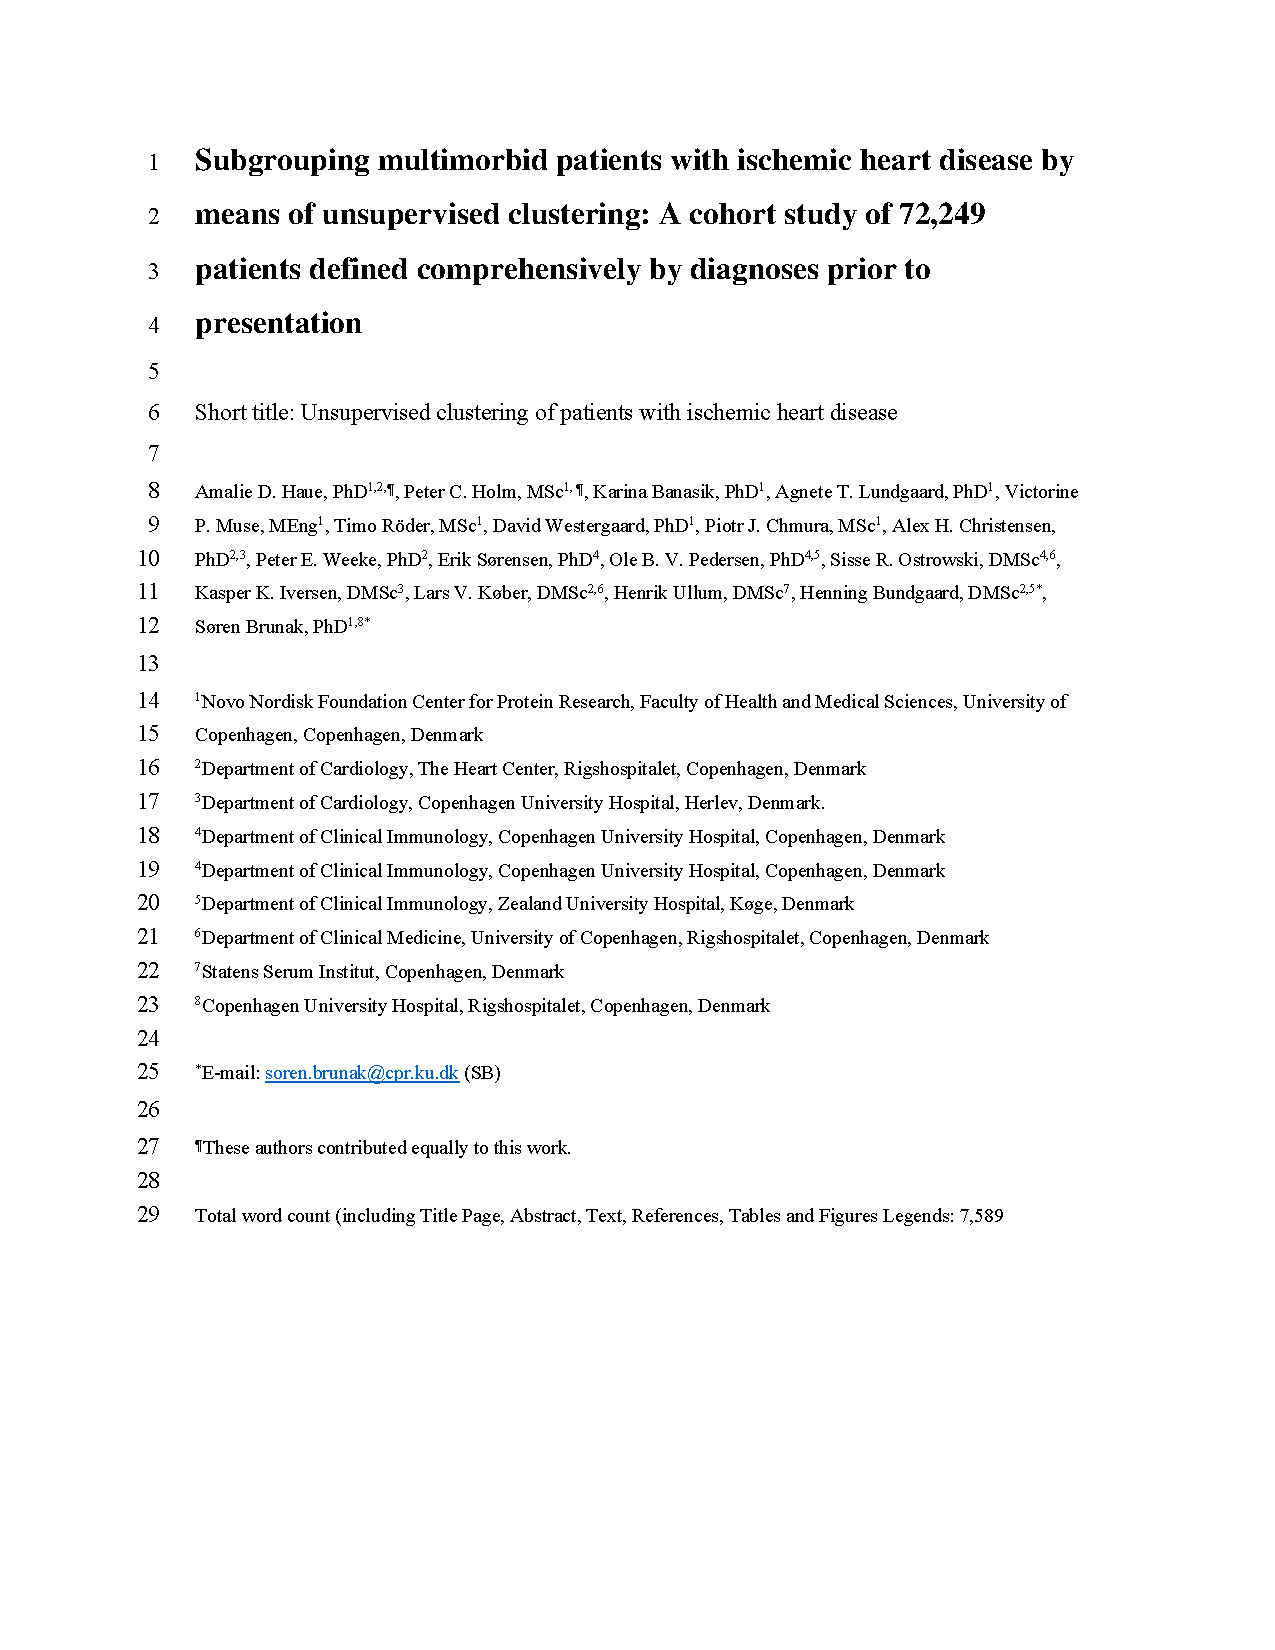
\includepdf[%
%     frame=true, scale=0.8, pages=-, pagecommand={}%
% ]{assets/paper1-clustering.pdf}

\end{document}
